\documentclass{beamer}
\usepackage[english,russian]{babel}
\usepackage[utf8]{inputenc}
\usepackage{amsmath}
\usepackage{hyperref}
\usetheme{Warsaw}
\usepackage{listings}
\usepackage{xcolor}
\usepackage{tikz}
\usetikzlibrary{graphs}
\usepackage{algpseudocode}

\lstset{
    frame=tb,
    tabsize=4,
    showstringspaces=false,
    numbers=left,
    commentstyle=\color{green},
    keywordstyle=\color{blue},
    stringstyle=\color{red},
    emph={baz},
    emphstyle=\textbf
}

\begin{document}

\title{SAT\\SMT solvers\newline 5. Linear arithmetic and Bit vectors}
\author{Roman Kholin}
\institute{Lomonosov Moscow State University}
\date{Moscow, 2023}

\begin{frame}
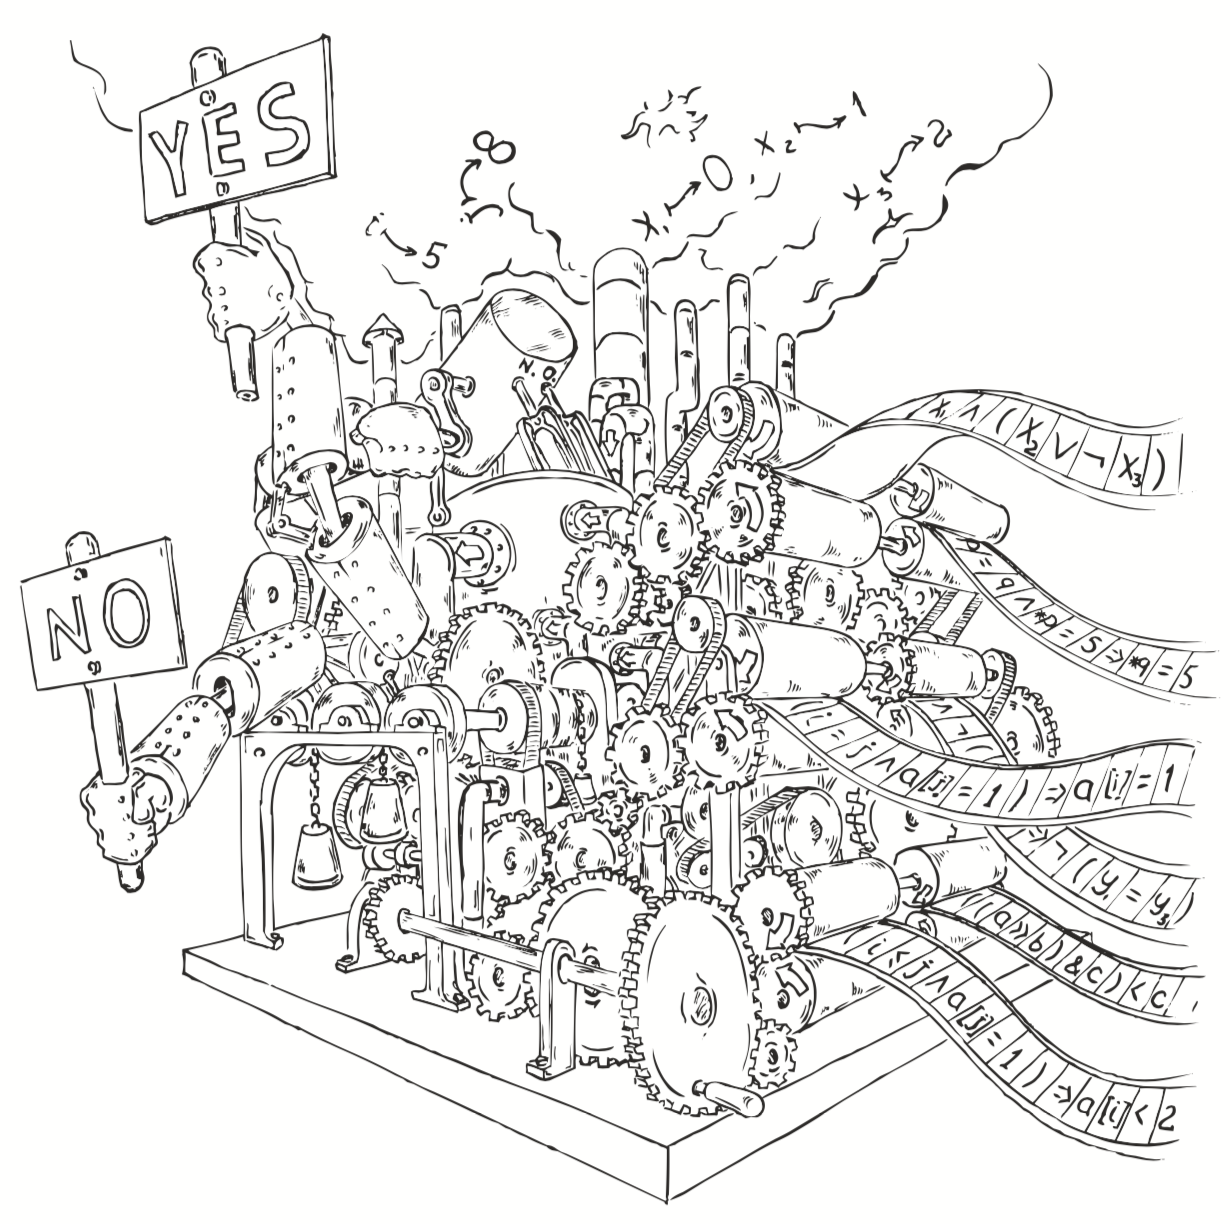
\includegraphics[scale=0.5]{../decision-procedure.png}
\end{frame}

\frame{\titlepage}

\begin{frame}{Linear arithmetic}
\begin{block}{Syntax}
\begin{itemize}
\item $formula: formula \wedge formula$ | $\lnot formula$ | $(formula)$ | $atom$
\item $atom : sum$ op $sum$
\item $op :$ $=$ | $\le$ | $<$
\item $sum : term$ | $sum + term$
\item $term : identifier$ | $constant$ | $constant$ identifier
\end{itemize}
$2z_1 + 3z_2 \le 5 \wedge z_2 + 5z_2 - 10z_3 \ge 6 \wedge z1 + z3 = 3$
\end{block}
\begin{block}{Decison procedure}
Simplex method
\end{block}
\end{frame}

\begin{frame}{Bit-Vector Arithmetic}
\begin{block}{Syntax}
\begin{itemize}
\item $formula: formula \wedge formula$ | $\lnot formula$ | $(formula)$ | $atom$
\item $atom : term$ $rel$ $term$ | $Boolean$-$Identifier$ | $term[constant]$
\item $rel : <$ | $=$
\item $term$ : $term$ op $term$ | $identifier$ | $\sim term$ | $constant$ | $atom?term:term$ | $term[constant : constant]$ | $ext(term)$
\item $op : + $| $-$ | $\cdot$ | $/$ | $<<$ | $>>$ | $\&$ | $|$ | $\bigoplus$ | $\circ$
\end{itemize}
\end{block}
\end{frame}

\begin{frame}{Motivation}
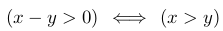
\includegraphics[scale=0.5]{mot1.png}\newline
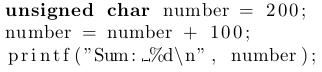
\includegraphics[scale=0.5]{mot2.png}\newline
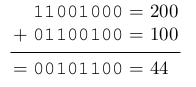
\includegraphics[scale=0.5]{mot3.png}
\end{frame}

\begin{frame}{Definitions}
\begin{block}{$\lambda$-notation}
$\lambda i \in \{0, \dots, l - 1\}.f(i)$
\end{block}
\begin{block}{Bit vector}
A bit vector b is a vector of bits with a given length l (or dimension):\newline
$b : \{0, \dots, l - 1\} \rightarrow \{0, 1\}$
\end{block}
\end{frame}

\begin{frame}{Definitions}
\begin{block}{Operator <<|>>}
$|_{[l]} : (bvec_l \times bvec_l ) \rightarrow bvec_l$\newline
$a | b ::= \lambda i.(a_i \vee b_i)$
\end{block}
\begin{block}{Binary encoding}
$x = \langle b\rangle_U$ - binary encoding, where\newline
$\langle\cdot\rangle_U : bvec_l \rightarrow \{0, \dots, 2l - 1\}$,\newline
$\langle b\rangle_U ::= \Sigma_{i = 0}^{l - 1}b_i\cdot 2^i$
\end{block}
\begin{block}{Two's complement}
$x = \langle b\rangle_S$ - two's complement, where\newline
$\langle\cdot\rangle_S : bvec_l \rightarrow \{-2^{l - 1}, \dots, 2{l-1} - 1\}$,\newline
$\langle b\rangle_S ::= -2^{l-1} \cdot b_{l-1} + \Sigma_{i = 0}^{l - 2}b_i\cdot 2^i$
\end{block}
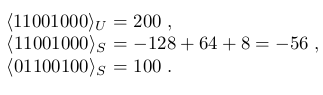
\includegraphics[scale=0.5]{Binary_encoding.png}\newline
\end{frame}

\begin{frame}{Definitions}
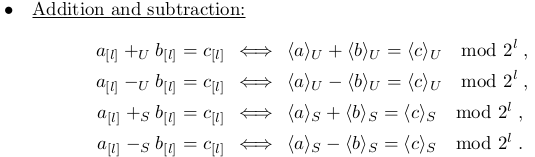
\includegraphics[scale=0.5]{Addition.png}\newline
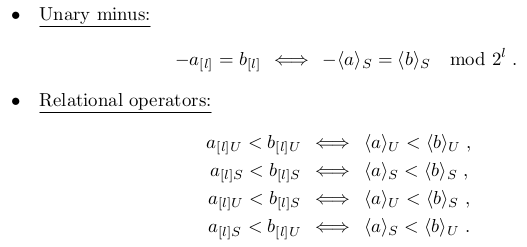
\includegraphics[scale=0.5]{Unary.png}\newline
\end{frame}

\begin{frame}{Definitions}
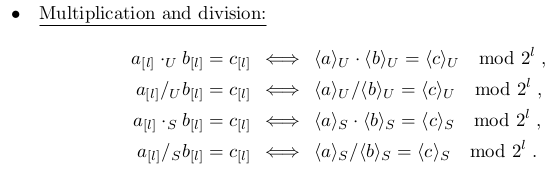
\includegraphics[scale=0.5]{Multiplication.png}\newline
\end{frame}

\begin{frame}{Definitions}
Extension:\newline
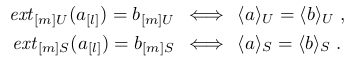
\includegraphics[scale=0.5]{ext.png}\newline
Shifting:\newline
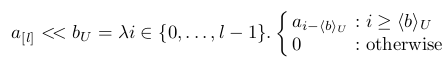
\includegraphics[scale=0.5]{sh0.png}\newline
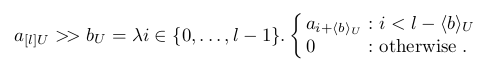
\includegraphics[scale=0.5]{sh1.png}\newline
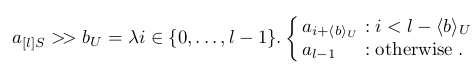
\includegraphics[scale=0.5]{sh2.png}\newline
\end{frame}

\begin{frame}{Algorithm}
\begin{itemize}
\item $T(\varphi)$ - the set of terms in $\varphi$
\item $e(t)$ - vector of variables for a given $t \in T(\varphi)$
\end{itemize}
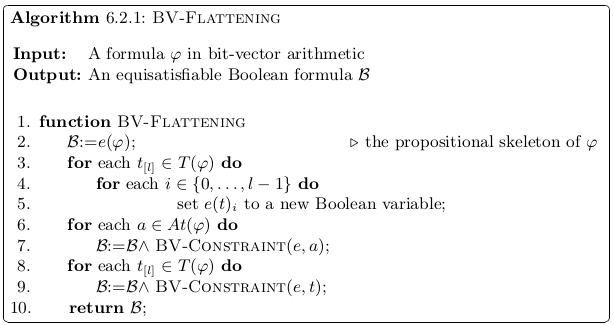
\includegraphics[scale=0.5]{algo.png}\newline
\end{frame}

\begin{frame}{Algorithm}
For all constant:\newline
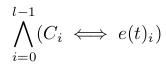
\includegraphics[scale=0.5]{skel.png}\newline
For <<|>> operator:\newline
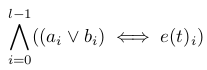
\includegraphics[scale=0.5]{or3.png}\newline
\end{frame}

\begin{frame}{Algorithm}
Full adder:\newline
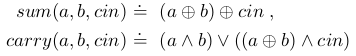
\includegraphics[scale=0.5]{sum1.png}\newline
Carry bits:\newline
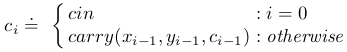
\includegraphics[scale=0.5]{sum2.png}\newline
Adder:\newline
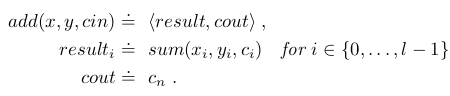
\includegraphics[scale=0.5]{sum3.png}\newline
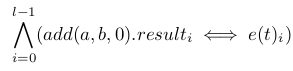
\includegraphics[scale=0.5]{sum4.png}\newline
\end{frame}

\begin{frame}{Relational Operators}
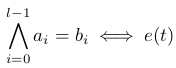
\includegraphics[scale=0.5]{rel1.png}\newline
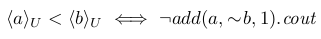
\includegraphics[scale=0.5]{rel2.png}\newline
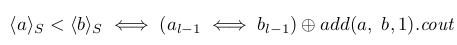
\includegraphics[scale=0.5]{rel3.png}\newline
\end{frame}

\begin{frame}{Shifts}
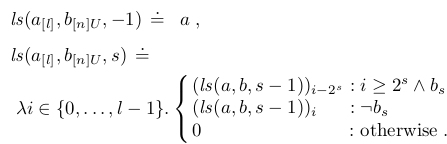
\includegraphics[scale=0.5]{ls.png}\newline
\end{frame}

\begin{frame}{Multiplication and Division}
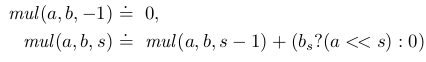
\includegraphics[scale=0.5]{mul1.png}\newline
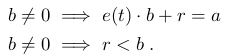
\includegraphics[scale=0.5]{div.png}\newline
\end{frame}

\begin{frame}{Some Operators Are Hard}
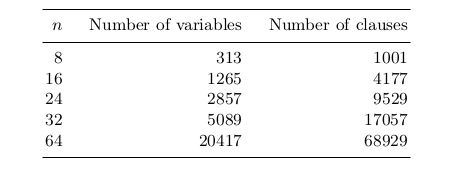
\includegraphics[scale=0.5]{Size.png}\newline
\end{frame}

\begin{frame}{Algorithm}
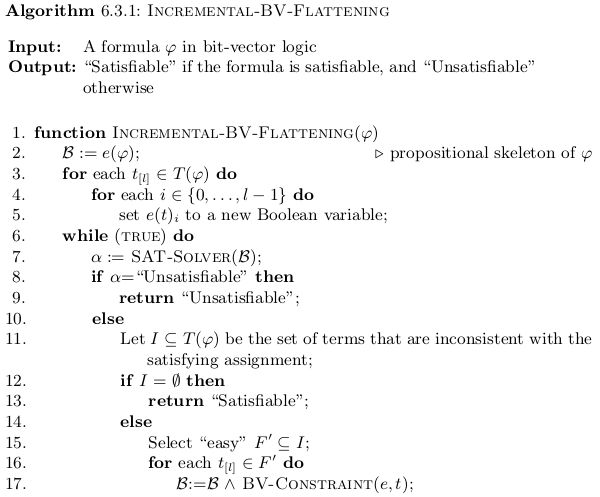
\includegraphics[scale=0.4]{algo2.png}\newline
\end{frame}

\begin{frame}{Fixed-Point Arithmetic}
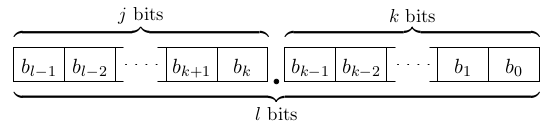
\includegraphics[scale=0.5]{fixpoint1.png}\newline
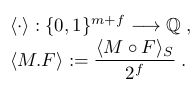
\includegraphics[scale=0.5]{fixpoint2.png}\newline
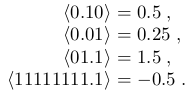
\includegraphics[scale=0.5]{fixpoint3.png}\newline
\end{frame}

\begin{frame}
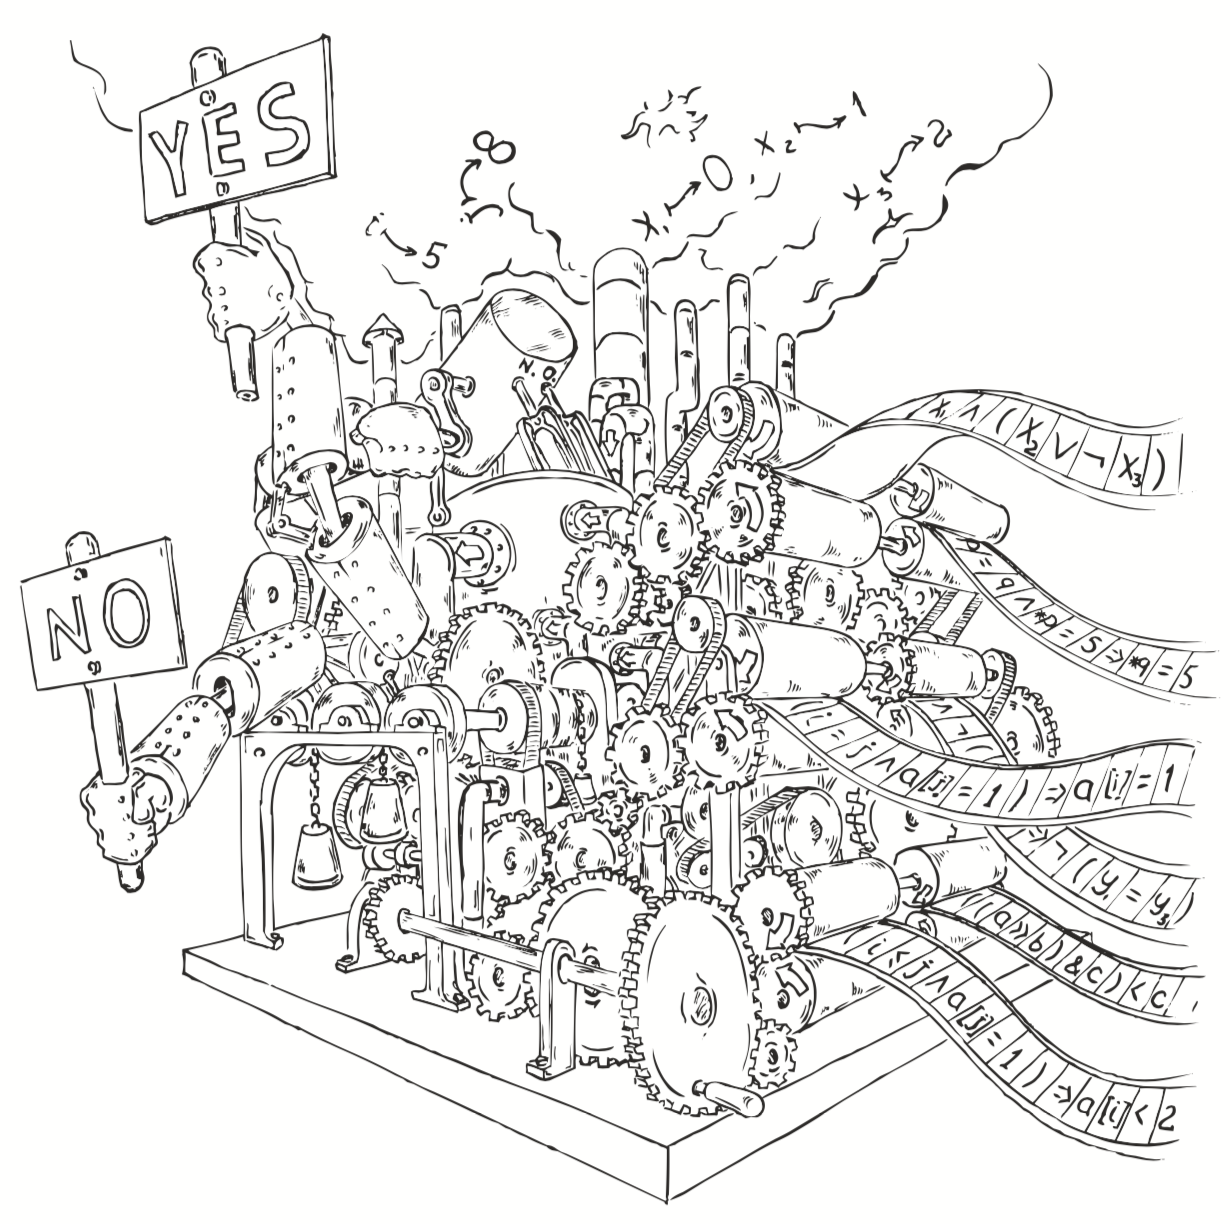
\includegraphics[scale=0.5]{../decision-procedure.png}
\end{frame}

\end{document}
